\chapter{Conclusion}\label{ch:conclusion}
\setlength{\epigraphwidth}{0.90\textwidth}
\epigraph{``We are all shaped by the tools we use, in particular: the formalisms we use shape our thinking habits, for better or for worse, and that means that we have to be very careful in the choice of what we learn and teach, for unlearning is not really possible.''}{\begin{flushright}--Edsger W. \citet{dijkstra2000answers}, \href{https://www.cs.utexas.edu/~EWD/transcriptions/EWD13xx/EWD1305.html}{\textit{Answers to questions from students of Software Engineering}}\end{flushright}}

In this thesis, we explored four different programming tools from software engineering for the development of intelligent systems, broadly addressing cognitive complexity arising in four phases of Royce's Waterfall method~\autoref{fig:waterfall_model}. These tools have varying degrees of practicality, from highly theoretical (e.g. adversarial testing of differentiable programs ~\autoref{ch:difftest}) to more pragmatic (e.g. containerization ~\autoref{ch:ducker}). In each chapter, we provide some motivating examples and use cases which demonstrate key deficiencies in state-of-the-art programming tools for intelligent systems and propose candidate solutions which address a few of those shortcomings. While we hope that intelligent system programmers (e.g. roboticists and machine learning practitioners) may derive some value from the tools themselves, our intention is to be \textit{illustrative} rather than \textit{prescriptive}.

In building tools and validating their effectiveness on toy applications, it is our hope that middleware and tool developers will carefully consider how software tools can reduce cognitive complexity. Tools can augment the cognitive capacity of humans to reason about facts in the presence of uncertainty~\citep{famelis2012partial}, and provide ergonomic debugging and visualization assistance (e.g. \autoref{ch:hatchery}). We also hope to convey the importance of notation. Good notation forces authors to think carefully about their abstractions, makes logical errors conspicuous, and allows the reader to more easily understand the implications of their own abstractions. We hope that the programming tools illustrated in this thesis will inspire developers to re-imagine the potential for computer-aided programming in the design of intelligent systems.

By complementing the cognitive abilities of human programmers -- who excel at creative problem solving and high-level abstract reasoning -- with the raw symbolic processing abilities of programming tools, we can accelerate the design~\autoref{ch:hatchery}, development~\autoref{ch:kotlingrad}, validation~\autoref{ch:difftest} and deployment~\autoref{ch:ducker} of intelligent systems in real-world applications. This process, we argue, is a virtous cycle which deserves domain-specific tools and practices due to the opportunities which intelligent systems afford and the unique interplay between human and machine intelligence.

As we start to engineer autonomous systems which take increasingly human decisions, software engineers and machine learning practitioners will play a critical role in shaping the behavior and dynamics of those systems. Language designers would do well to consider the role of human and machine intelligence and the value of tools in facilitating that relationship. This requires domain-specific models to communicate human knowledge i.e. differentiable programming as well as expert systems in the form of types which help to reason about compositionality and correctness (\autoref{ch:kotlingrad}). Finally, ensuring software artifacts are reproducible will require build systems and best practices in developer operations (e.g. \autoref{ch:ducker}).

Traditional software engineering prescribes a rigorous process model and testing methodology~\autoref{fig:waterfall_model} which has guided generations of software projects. To become a true engineering discipline, the machine learning community will need to develop a more rigorous methodology for building intelligent systems. Machine learning models are usually trained on \textit{objective functions}, which are typically one- or low-dimensional functions for measuring the overall performance of a system, typically outputting a scalar value known as an \textit{error} or \textit{loss}. In practice, we care about a multiobjective set of criteria~\citep{censi2015mathematical}, including energy efficiency~\citep{paull2010novel}, memory~\citep{memory2013mitliagkas}, re/usability~\citep{breuleux2017automatic,deleu2019torchmeta}, predictability~\citep{turner2017well}, latency~\citep{ravanelli2018twin}, robustness~\citep{pineau2003policy}, explainability~\citep{turner2016model}, traceability~\citep{guo2017semantically, tsirigotis2018orion}, un/certainty~\citep{diaz2018interactive}, simplicity~\citep{kastner2019representation}, trustworthiness~\citep{xu2017efficient}, transferability~\citep{mehta2019active}, scalability~\citep{luan2019break} and many other factors.

In traditional software engineering, it is reasonable to assume those implementing a new system have some implicit domain knowledge and are well-intentioned human beings working towards a common goal -- given a coarse description, they can fill in the blanks. However when building an intelligent system, we would be safer to assume the requirements are implemented by a na\"ive but crafty genie. Given some data and an optimization metric, it will take every available shortcut to satisfy our desired criteria. If we are not careful about correctly specifying the requirements, this entity will create a solution that simply does not work (in the best case), or might appear to work but is subtly cursed~\citep{bellman1957dynamic}.

When building an intelligent system developers must carefully ask, ``What is the expected behavior of the system we are designing?'' This question is often very troublesome, for the requirements cannot be loose specifications, but precise constraints on the solution set. Fully specifying the requirements is indistinguishable from implementing the system -- with the right language abstractions (e.g.\ declarative programming), requirements and implementation can even take the same notation (e.g. SQL, Prolog). But how can we be assured the resulting system satisfies our requirements? Humans can drive a car, but have enormous difficulty describing an algorithm for driving. Labeling the data by hand is too expensive. Exhaustive verification is right out the window.

For example, in the design of an online ad recommendation system, we can optimize for various criteria such as click rate, engagement, and sales conversion. So long as we can measure these parameters, modern function approximators can optimize for any single criterion or combination thereof (\autoref{eq:moo_spec}). Much of the work involved in machine learning is designing representations which are suitable for downstream tasks and loss functions which accurately measure performance on those tasks. For example, by na\"ively optimizing for click rate, we create an artificial market for click bots. Similarly, in self-driving vehicles, we often want to optimize for passenger safety. However, doing so na\"ively will train a vehicle that never moves, or always yields to passing vehicles. Building representations and loss functions which capture the full range of objectives can be a painstaking process.

\begin{figure}
    \centering
    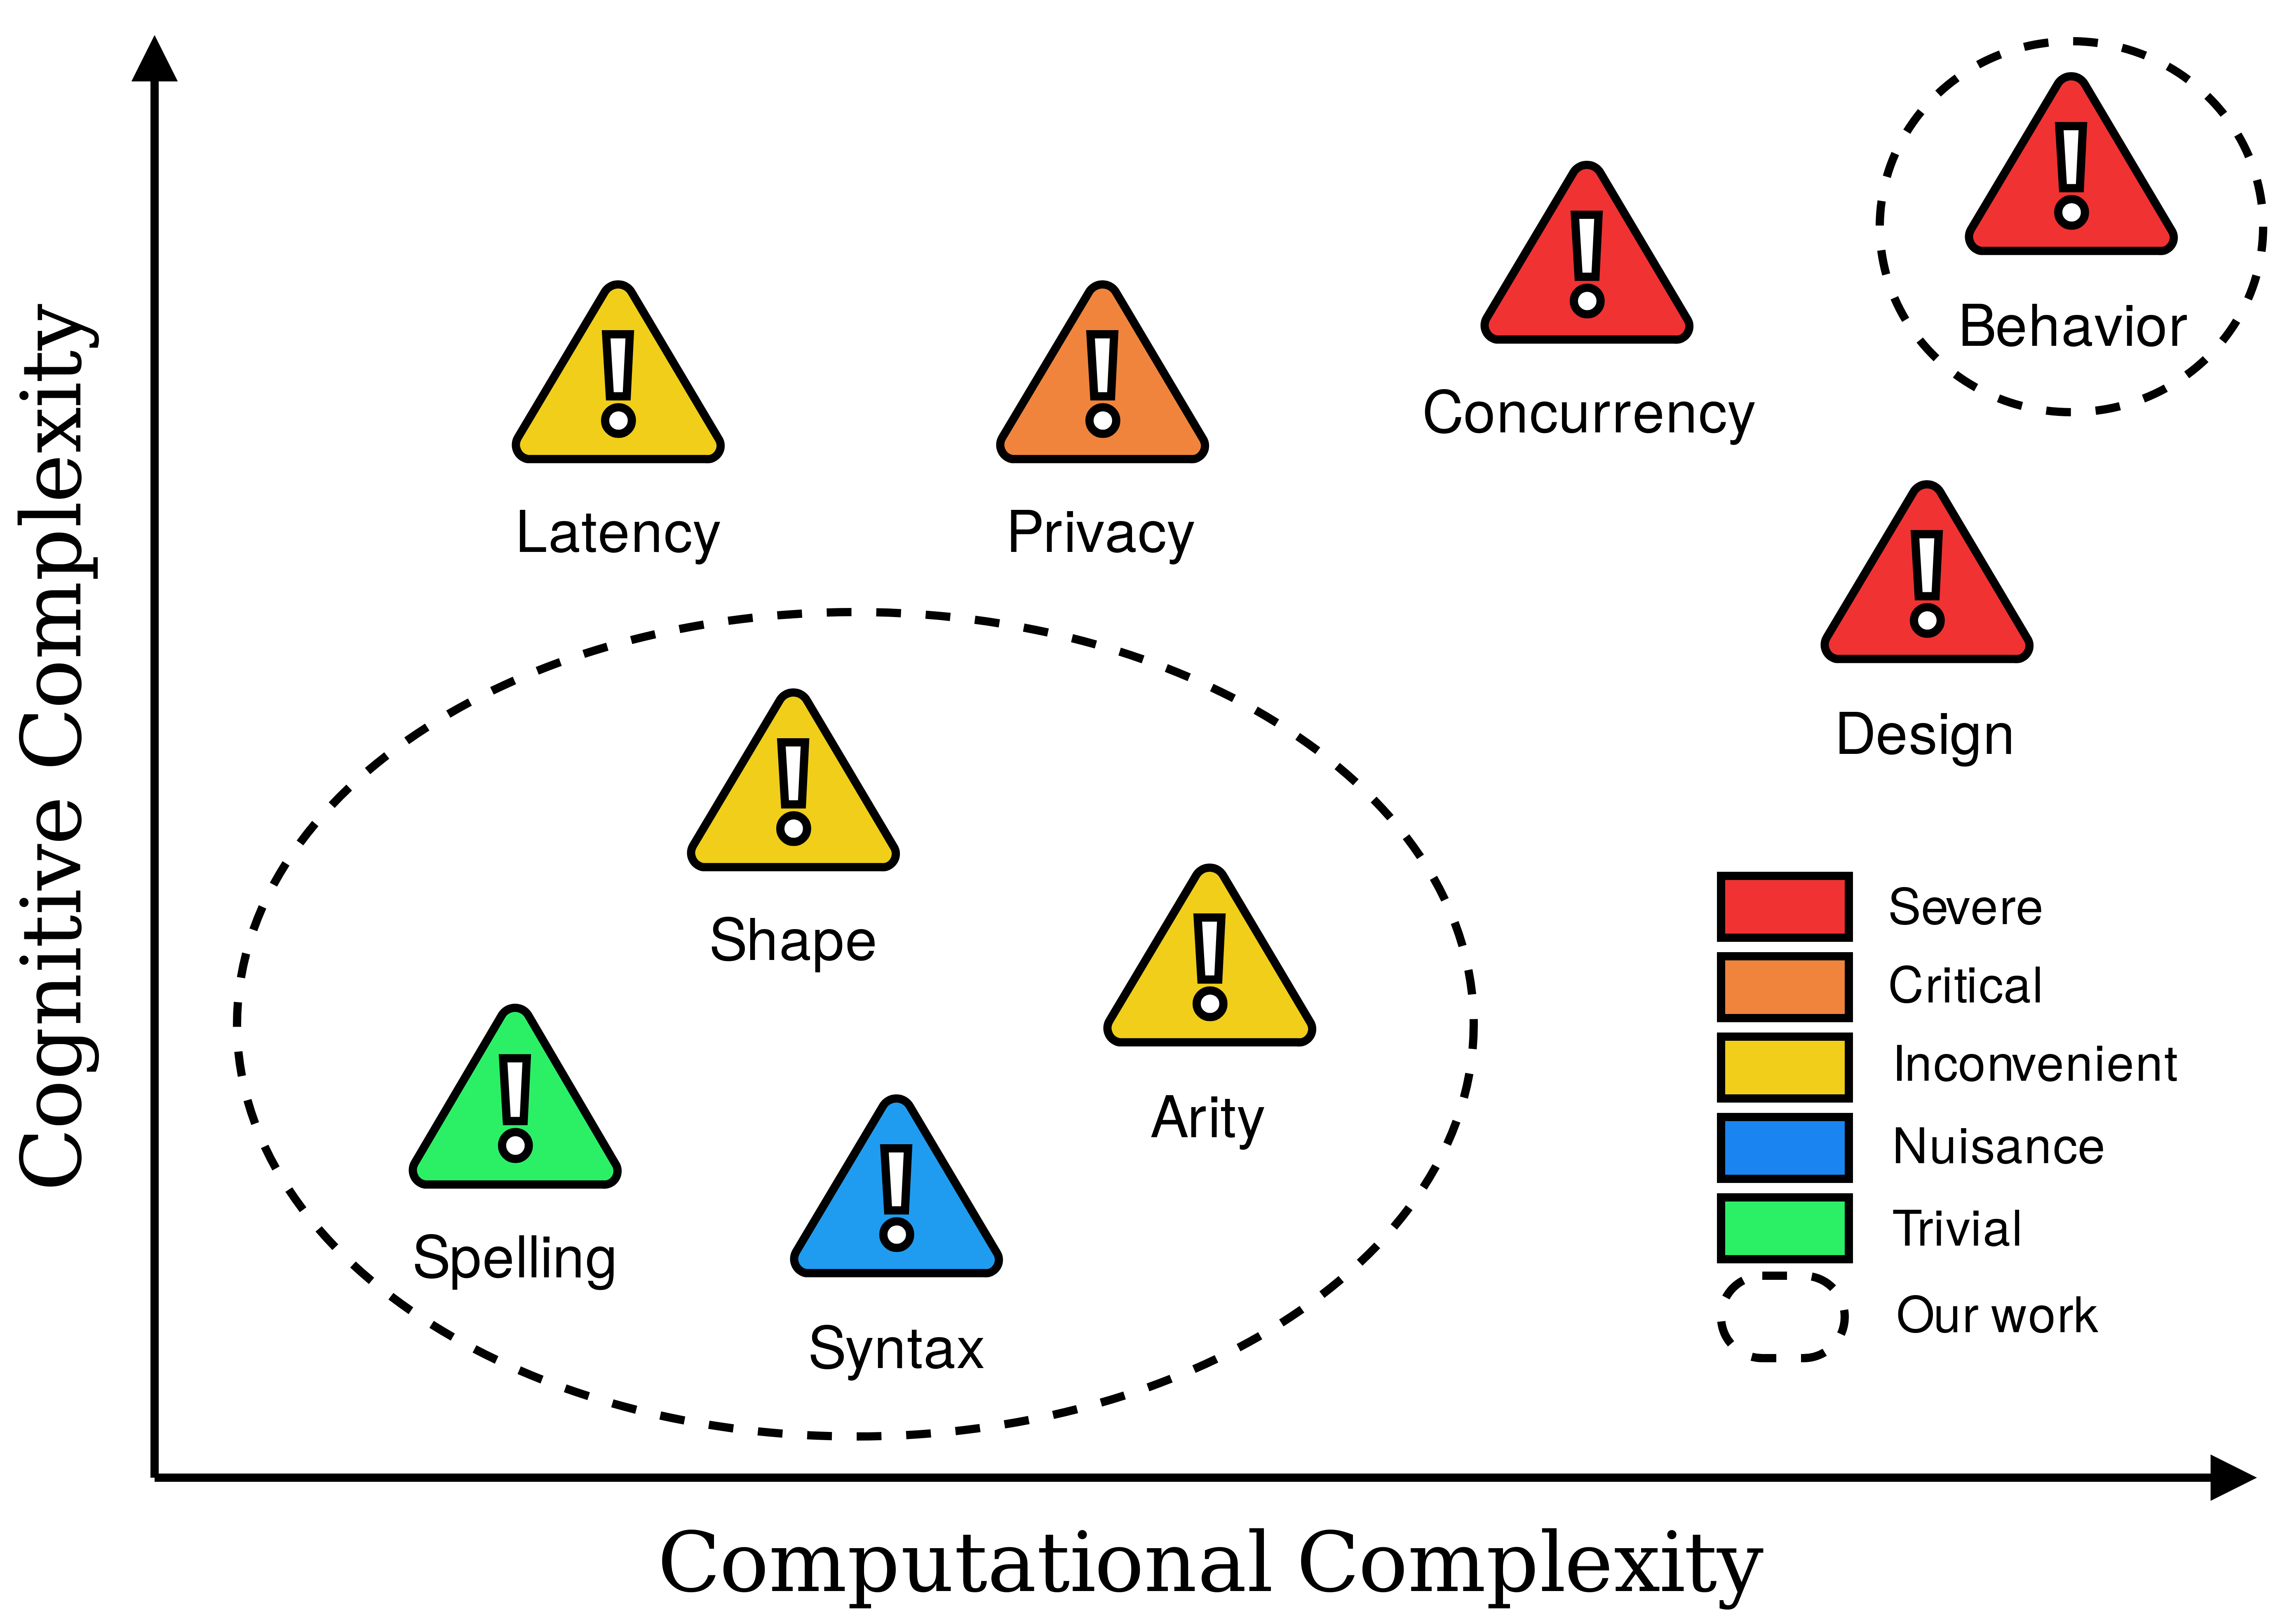
\includegraphics[width=0.60\textwidth]{../figures/verification_complexity.png}
    \caption{Complexity of detecting various types of programming errors.}
    \label{fig:verification_complexity}
\end{figure}

Type systems, compilers and fuzzers are all part of a broader class of validation and verification tools. The goal of these tools is to trade cognitive complexity for computational complexity. Some errors (e.g. syntactical errors), are minor nuisances and can be detected with a good incremental parser (\autoref{subsec:the-parser}). Others, as shown in~\autoref{fig:verification_complexity}, have higher cognitive complexity but can be detected by spending computation. We argue this computational cost is often justified as computation is cheap and undetected bugs can have catastrophic consequences. Spending computation frees up valuable cognitive resources which are more wisely spent on more challenging tasks. Studies have shown that bugs detected early in development are more likely to be fixed~\citep{distefano2019scaling} -- saving minutes in development could save lives during operation.

Where fuzz testing remains an economical alternative. As we show in \autoref{sec:prob_ad_test}, by making practical assumptions about the model and oracle, we can spend a fixed computational budget to detect more severe errors with lower fiscal and computational overhead.

Learning capabilities will play a crucial role in autonomous systems. As today's engineers begin to incorporate learning in tomorrow's safety-critical robotic systems, we believe the increased assurance provided by intelligent validation and verification tools will be indispensable for the widespread deployment of these complex adaptive cyberphysical systems.